\documentclass[12pt]{article}

% The preceding line is only needed to identify funding in the first footnote. If that is unneeded, please comment it out.
\usepackage{cite}
\usepackage{amsmath,amssymb,amsfonts}
\usepackage{algorithmic}
\usepackage{graphicx}
\usepackage{textcomp}
\usepackage{xcolor}
\usepackage{multirow}

\usepackage[utf8]{inputenc}
\usepackage[T1]{fontenc}
\usepackage[english]{babel}
\usepackage[backend=biber,style=ieee,autocite=inline]{biblatex}
\bibliography{ref.bib}
\DefineBibliographyStrings{english}{%
  bibliography = {References},}


\title{Assignment 1}
\author{Ivan Efremov}
\date{March 2022}

\begin{document}

\maketitle

\section{Task 1}
\subsection{Task 1.1}
We can see, that vectors $v_i$, $w_i$ form the plane. So this vectors  should not lie in the same line to form a plane.
If one of the vector of second plane not lie in the first plane, first and second planes would intersect, otherwise they are parallel.  

So we can from two matrices A1 = [v1 w1 v2] and A2 = [v1 w1 w2]. If one of them is invertible (has independent columns), planes would intersect. 

The code you can find in Task\string_1\string_1.m

\begin{figure}[h]
    \centering
    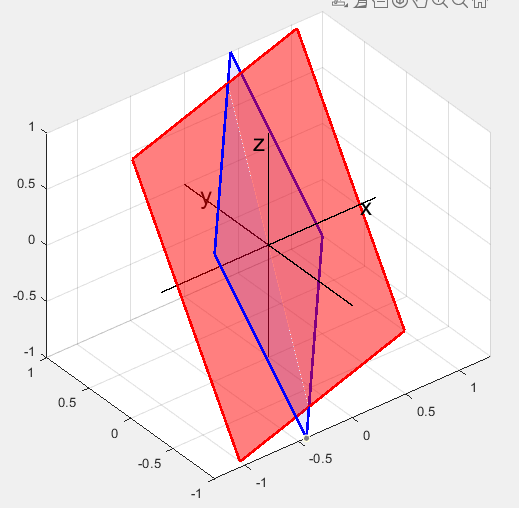
\includegraphics[scale=0.4]{Task_1_1.png}
    \caption{Intersection of 2 planes}
    \label{fig:my_label}
\end{figure}

\subsection{Task 1.2}
Find representation in form $n*(r-r_0) = 0$.  

n is perpendicular to the plane, so it's perpendicular to vectors v and w - left null space of matrix [v w].  

$r0$ is equal to any point in that plane. So let it be just p. 

You can find a code in Task\string_1\string_2.m

\begin{figure}[h]
    \centering
    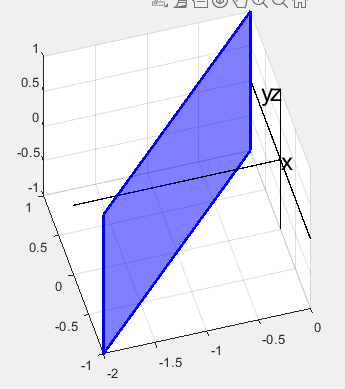
\includegraphics[scale=0.5]{Task_1_21.png}
    \caption{First plane in task 1.2}
    \label{fig:my_label}
\end{figure}

\begin{figure}[h]
    \centering
    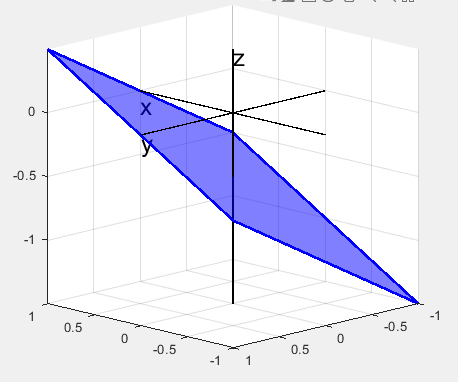
\includegraphics[scale=0.5]{Task_1_22.png}
    \caption{Second plane in task 1.2}
    \label{fig:my_label}
\end{figure}
\subsection{Task 1.3}
Line vector is equal to normal of the plane. To find a projection I am using the formula of projection: $g_{proj} = n * (n^T * n)^{-1} * n^T * g$

You can find a code in Task\string_1\string_3.m

\begin{figure}[h]
    \centering
    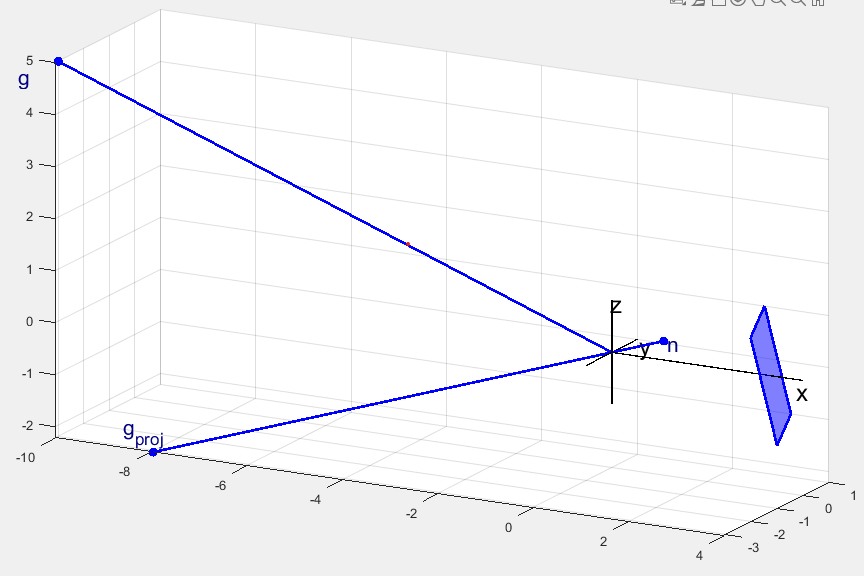
\includegraphics[scale=0.35]{Task_1_3.png}
    \caption{Solution of the task 1.3}
    \label{fig:my_label}
\end{figure}

\subsection{Task 1.4}
In this task I decompose vector g on two vectors: projection vector to plane s and perpendicular vector to the plane s equals to distance to that plane (n vector). So symmetrical point will compute as $g^* = g_{proj} - n$

You can find a code in Task\string_1\string_4.m

\begin{figure}[!h]
    \centering
    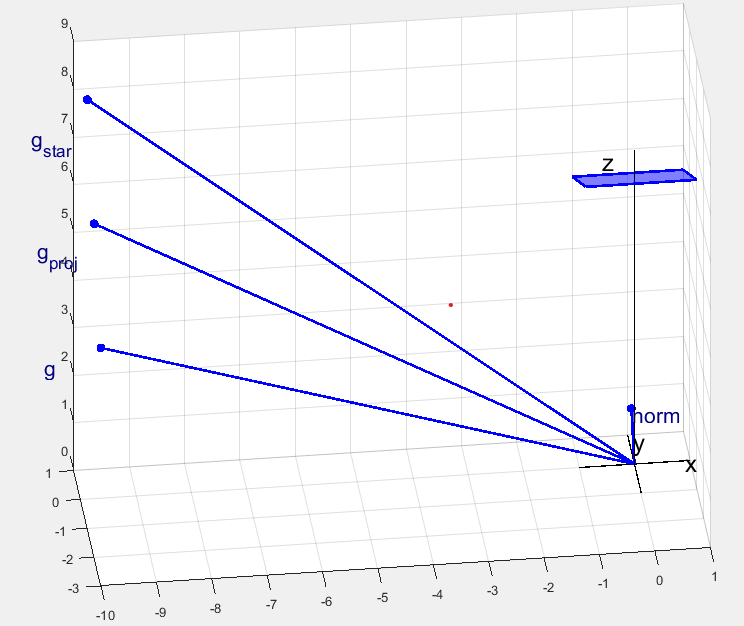
\includegraphics[scale=0.35]{Task_1_4.png}
    \caption{Solution of the task 1.4}
    \label{fig:my_label}
\end{figure}

\section{Task 2}
To get a basis of V, we should just compute null space of the matrix. This function is available in matlab.

Finding orthogonal projection onto V  and onto the orthogonal compliment of V is similar as in task 1.4.

To recover g: $g = g^{\perp} + g^{||}$. To prove that $g^{\perp}$ and $g^{||}$ are perpendicular we can take scalar multiplication of this vectors, which should be equal to zero.

You can find a code in Task\string_2.m

\begin{figure}[!h]
    \centering
    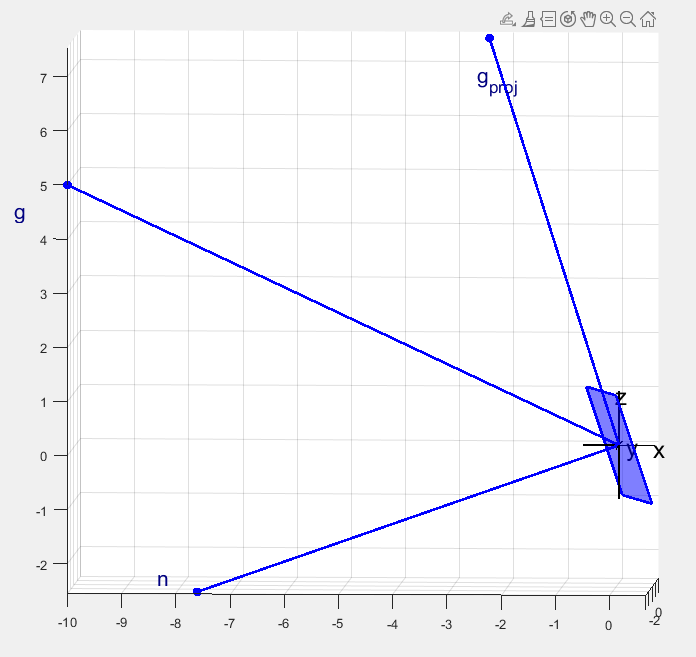
\includegraphics[scale=0.5]{Task_2.png}
    \caption{Solution of the task 2}
    \label{fig:my_label}
\end{figure}

\section{Task 3}

To rearrange optimization problem in another form we should use the following values:

\vspace{\bigskipamount}
H = 
\begin{bmatrix}
    1       & 0  \\
    0       & 8 \\
\end{bmatrix} 

c = 
\begin{bmatrix}
    0       & -32  \\
\end{bmatrix}
\vspace{\bigskipamount}

c0 = 60

\vspace{\bigskipamount}

A = 
\begin{bmatrix}
    1       & 1  \\
    1       & 2  \\
    -1       & 0  \\
    0       & -1  \\
    1       & 1  \\
\end{bmatrix}

\vspace{\bigskipamount}

b = 
\begin{bmatrix}
    6     \\
    8     \\
    0    \\
    0     \\
    9     \\
\end{bmatrix}

\vspace{\bigskipamount}

A solution on CVXPY and visualization you can find in Task\string_3.ipynb


\end{document}